\chapter{L'offre \og plateformes d'intégration continue \fg}
\label{section:pic}

\paragraph{}
Quand on sait que 70\% des projets informatiques ne respectent pas le planning initial ou se transforment en échecs~\cite{echec}, on cherche par tous les moyens à réduire les facteurs responsables.
Le manque de qualité logicielle et de suivi de projet en font évidemment parti.
Alors que ces domaines étaient encore un marché de niche il y a quelques temps de cela, aujourd'hui, de plus en plus de clients et de DSI\footnote{Directions de Services Informatiques} commencent à s'en préoccuper et à remettre en cause les méthodes classiques de gestion de projets informatiques.
C'est aussi l'occasion de tenter de pérenniser les développements qui au fil du temps perdent toujours plus en maintenabilité.

\paragraph{}
La qualité logicielle et le suivi de projets informatiques deviennent donc un véritable enjeu actuel.
Les entreprises doivent alors se doter de nouveaux process et de nouveaux outils. 
Elles peuvent les acquérir en faisant notamment appel à des prestations de conseil dans le domaine, qui font entre autres intervenir des notions de gestion de projet et de bonnes pratiques en terme de génie logiciel.
Au-delà de ça, les nouveaux outils doivent être mis en place et intégrés aux infrastructures systèmes existantes.

\paragraph{}
C'est ainsi que la \abusys{} de \asmile, sous l'impulsion de \agulet, s'est positionnée sur ce marché.
Une offre open source a été construite pour répondre au besoin de A à Z, de l'installation des outils au conseil sur leur utilisation, en passant par leur configuration personnalisée.


\section{Intérêt des méthodes agiles}

\paragraph{}
Les méthodes agiles sont très répandues dans les communautés du logiciel libre.
Les programmes y sont souvent développés en en suivant les principes.
Raison de plus pour que \asmile{}, leader sur le marché de l'open source, fasse la promotion de l'agilité après des entreprises.


\paragraph{}
Les méthodes agiles partent du constat que les spécifications initiales du client sont souvent \og volatiles \fg, dans le sens où elles évoluent relativement vite dans le temps et qu'elles souffrent régulièrement d'imprécision.
Les méthodes lourdes classique de développement impliquant spécifications, réalisation puis recette par le client se révèlent donc inadaptées.
Au contraire, il faut privilégier des cycles de développement courts qui apportent la flexibilité nécessaire pour pouvoir corriger rapidement à coût moindre les éventuelles erreurs de spécification ou de conception.

L'organisation du développement épouse alors deux aspects :

\begin{itemize}
	\item le côté itératif, car le logiciel est créé sur plusieurs cycles d'une durée relativement courte ;
	\item l'aspect incrémental, car chaque nouveau cycle améliore les fonctionnalités du précédent.
\end{itemize}


\paragraph{}
En outre, le Manifeste Agile~\cite{agile}, considéré comme l'acte généralisateur des méthodes agiles, invite à adopter un certain nombre de valeurs :

\begin{itemize}
	\item il faut privilégier les personnes et les interactions plutôt que de suivre aveuglément des procédures et d'être dirigé par ses outils ;
	\item la création régulière de jalons fonctionnels est une priorité pour garder cons\-tam\-ment à l'idée ce qu'est et ce que va être le produit final ;
	\item la clé est la collaboration étroite avec le client, alors que l'on a traditionnellement tendance à respecter un contrat et à suivre des spécifications initiales ;
	\item le client et le prestataire réalisateur doivent tous deux être flexible et accepter le changement.
\end{itemize}


\paragraph{}
Les méthodes agiles sont parfois difficiles à mettre en place car elles sont souvent en rupture avec les processus existants de l'entreprise.
De plus, la flexibilité requise peut être confondue avec un défaut d'organisation, ce qui amène inévitablement à des résultats catastrophiques.
Au contraire, de bons outils adaptés sont nécessaires pour effectuer un vrai suivi du projet.
Ils doivent permettre de tracer de façon transparente les changements et d'améliorer la communication entre les différents acteurs du projet.



\section{La gestion de projet agile}

\subsubsection{Outil : Redmine}

\subsubsection{Outil : JIRA}

\subsubsection{Mission : Formation JIRA chez Rexel}

\subsubsection{Mission : Développement Redmine}

- Développement de plugins

- Contribution au core



\section{Gestion de versions du code source}
\label{section:pic-source}

\subsection{Outils}

\subsubsection{Subversion}

\subsubsection{Git}

\subsection{Missions}

\subsubsection{Formation Subversion chez Rexel}

\subsubsection{Synchronisation de mirroirs SVN pour Rexel}

\subsubsection{Plan de formation Git}



\section{Tests des applications}

Tester l'application est une condition nécessaire si l'on veut s'assurer de sa qualité.
Les tests manuels par les développeurs ou les utilisateurs sont loin d'être suffisants : il existe bien trop de cas à vérifier.
Pour répondre à ce problème d'exhaustivité, il est possible de mettre en place des tests automatiques et programmables.
Aussi, on peut distinguer deux types de tests : les tests \emph{unitaires} et les tests \emph{fonctionnels}.



\subsection{Tests unitaires}

Pour expliquer ce qu'est ce premier type de tests, je m'en réfère à l'excellent article Wikipédia à ce sujet.~\cite{unit}

\begin{quotation}
Le test unitaire est un procédé permettant de s'assurer du fonctionnement correct d'une partie déterminée d'un logiciel ou d'une portion d'un programme (appelée \og unité \fg{} ou \og module \fg).

On écrit un test pour confronter une réalisation à sa spécification. Le test définit un critère d'arrêt (état ou sorties à l'issue de l'exécution) et permet de statuer sur le succès ou sur l'échec d'une vérification.
Grâce à la spécification, on est en mesure de faire correspondre un état d'entrée donné à un résultat ou à une sortie.
Le test permet de vérifier que la relation d'entrée/sortie donnée par la spécification est bel et bien réalisée.

Il s'agit pour le programmeur de tester un module, indépendamment du reste du programme, ceci afin de s'assurer qu'il répond aux spécifications fonctionnelles et qu'il fonctionne correctement en toutes circonstances.
Cette vérification est considérée comme essentielle, en particulier dans les applications critiques.
Elle s'accompagne couramment d'une vérification de la couverture de code (évaluation de la couverture structurelle), qui consiste à s'assurer que le test conduit à exécuter l'ensemble (ou une fraction déterminée) des instructions présentes dans le code à tester.

L'ensemble des tests unitaires doit être rejoué après une modification du code afin de vérifier qu'il n'y a pas de régressions (l'apparition de nouveaux dysfonctionnements).
\end{quotation}



\subsection{Tests fonctionnels}

Les tests fonctionnels diffèrent des tests unitaires du point de vue qu'ils vérifient les fonctionnalités de l'application.
Leur portée s'éloigne ainsi du code et devient globale à l'application.

Au niveau d'un site web, par exemple, un test fonctionnel consiste à naviguer à l'intérieur, en cliquant sur des liens, en remplissant des formulaires, ou encore en vérifiant si divers éléments d'une page sont bien présents.

Ce type de test prend tout son intérêt quand il s'agit de tester un cas d'utilisation typique d'une application par ses utilisateurs finaux.
En reproduisant un ensemble significatif des scénarios utilisateurs sous forme de tests fonctionnels, on peut alors s'assurer du bon fonctionnement global du programme, quels que soient les changement de code entrepris.



\subsection{Outils}

\subsubsection{Librairies de tests unitaires}

\paragraph{}
Chaque langage de programmation dispose de sa librairie pour rédiger des tests unitaires, si ce n'est plus.
Par exemple, on va trouver JUnit pour Java, PHPUnit ou Lime pour PHP, CppTest pour C++, etc.

\paragraph{}
La façon de rédiger des tests est souvent la même malgré les différences entre langages de programmation.
Pour une fonction, ce processus est répété pour chaque ensemble de paramètres d'entrée à tester :

\begin{enumerate}
	\item le contexte d'exécution est défini à travers des définition de variable est des appels de fonctions ;
	\item la fonction à tester unitairement est appelée, avec en entrée des paramètres choisis pour être des cas classiques ou des cas limites ;
	\item le retour de la fonction (voire même le déclenchement d'exception) est comparé à un résultat attendu issu des spécifications.
\end{enumerate}

Ainsi, chaque fonction à tester est exécutée plusieurs fois de suite avec des paramètres d'entrée différents afin de bien couvrir tous les cas.



\subsubsection{Selenium}

\paragraph{}
Selenium est un outil de tests fonctionnels pour les sites web.
Disponible sous la forme d'une extension pour le navigateur web Firefox, il enregistre l'enchaînement des liens cliqués pour naviguer de page en page.
Quand le test est joué, si une page du scénario ne s'affiche pas, on considère que c'est un échec.

Un autre test souvent utilisé est la vérification de la présence d'un texte sur une page.
C'est très pratique dans le cas où l'on veut vérifier la présence ou non d'erreurs après la soumission d'un formulaire, par exemple.

Enfin, le jeu de tests peut être sauvé dans un fichier afin de pouvoir être rejoué ultérieurement.

\paragraph{}
La \reffigure{pic-tests:selenium} montre une capture d'écran de Selenium.

\begin{figure}
	\centering
	\includegraphics[width=7cm]{pic/selenium-ide}
	\caption{Selenium en action}
	\label{figure:pic-tests:selenium}
\end{figure}



\subsection{Missions}

\subsubsection{Formation Selenium chez Spir}

\paragraph{}
Spir est un éditeur de journaux de petites annonces qui édite aujourd'hui des sites \ainternet{} comme Top Annonces ou Logic Immo.
Pour améliorer son processus qualité, le client désire s'équiper d'un outil permettant de jouer automatiquement des tests fonctionnels.

\paragraph{}
Je me suis alors rendu dans leurs locaux avec \agulet{} pour leur présenter l'outil Selenium.
C'est une formation que j'ai préparée en amont moi-même et que nous avons présenté au client en duo.



\section{Intégration continue}

\subsection{Outils}

\subsubsection{Hudson/Jenkins}

\subsection{Missions}

\subsubsection{paramétrage de la PIC de Spir}

\subsubsection{Formation Jenkins chez Spir}



\section{Bilan}

\paragraph{}
Finalement, \asmile{} fournit une offre complète d'intégration système autour des méthodes agiles et de l'intégration continue.
Le client peut suivre son projet avec Redmine, manipuler son code source avec Subversion tout en conservant un historique de l'ensemble des changements effectués, et enfin tester son application en continu avec Jenkins.
Il est accompagné par les ingénieurs système de \asmile{} qui peuvent lui proposer une prestation de conseil.

\paragraph{}
La \reffigure{pic:bilan} offre une vue d'ensemble de l'offre.

\begin{figure}
	\centering
	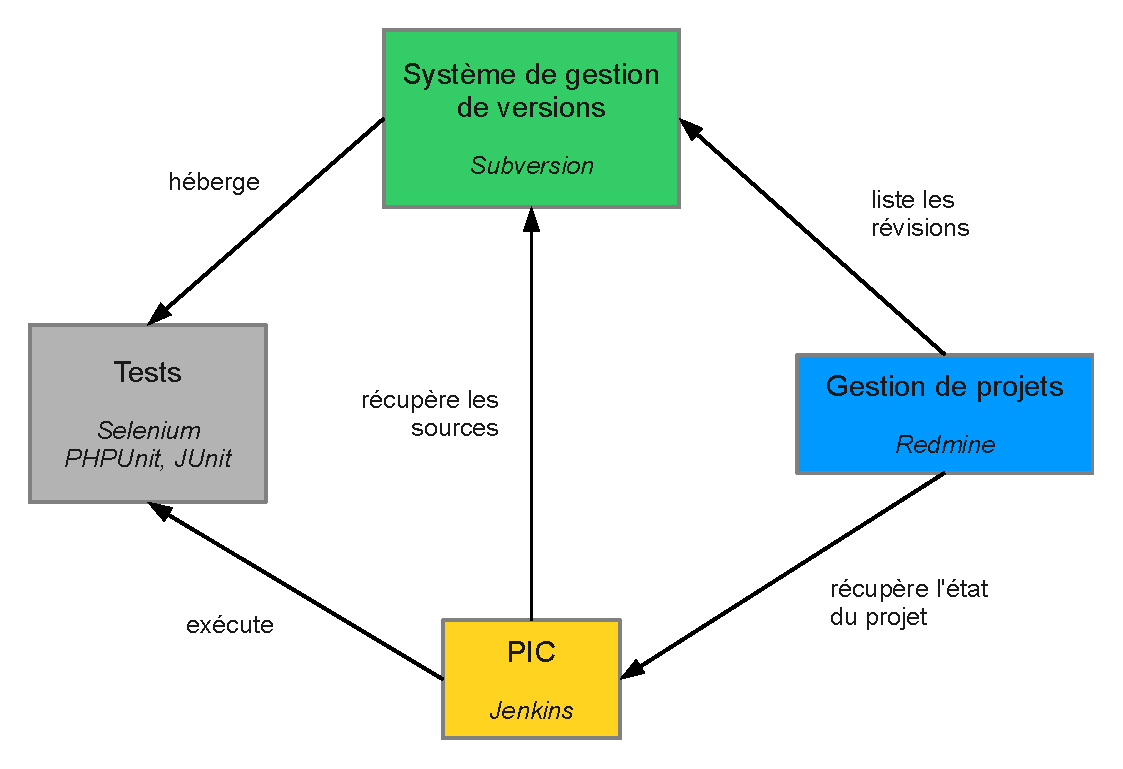
\includegraphics[width=14cm]{pic/bilan}
	\caption{Vue d'ensemble de l'offre \og Plateformes d'intégration continue \fg}
	\label{figure:pic:bilan}
\end{figure}



